\documentclass[10pt,a4paper]{article}
\usepackage[utf8]{inputenc}
\usepackage[T1]{fontenc}
\usepackage[ngerman]{babel}
\usepackage{amsmath}
\usepackage{amsfonts}
\usepackage{amssymb}
\usepackage{graphicx}


\author{Gruppe 02}
\title{Pflichtenheft}
\begin{document}

	\subsection{Adminbereich}
	\subsubsection{Sperren Teilnehmer}
	\begin{figure}[h]
		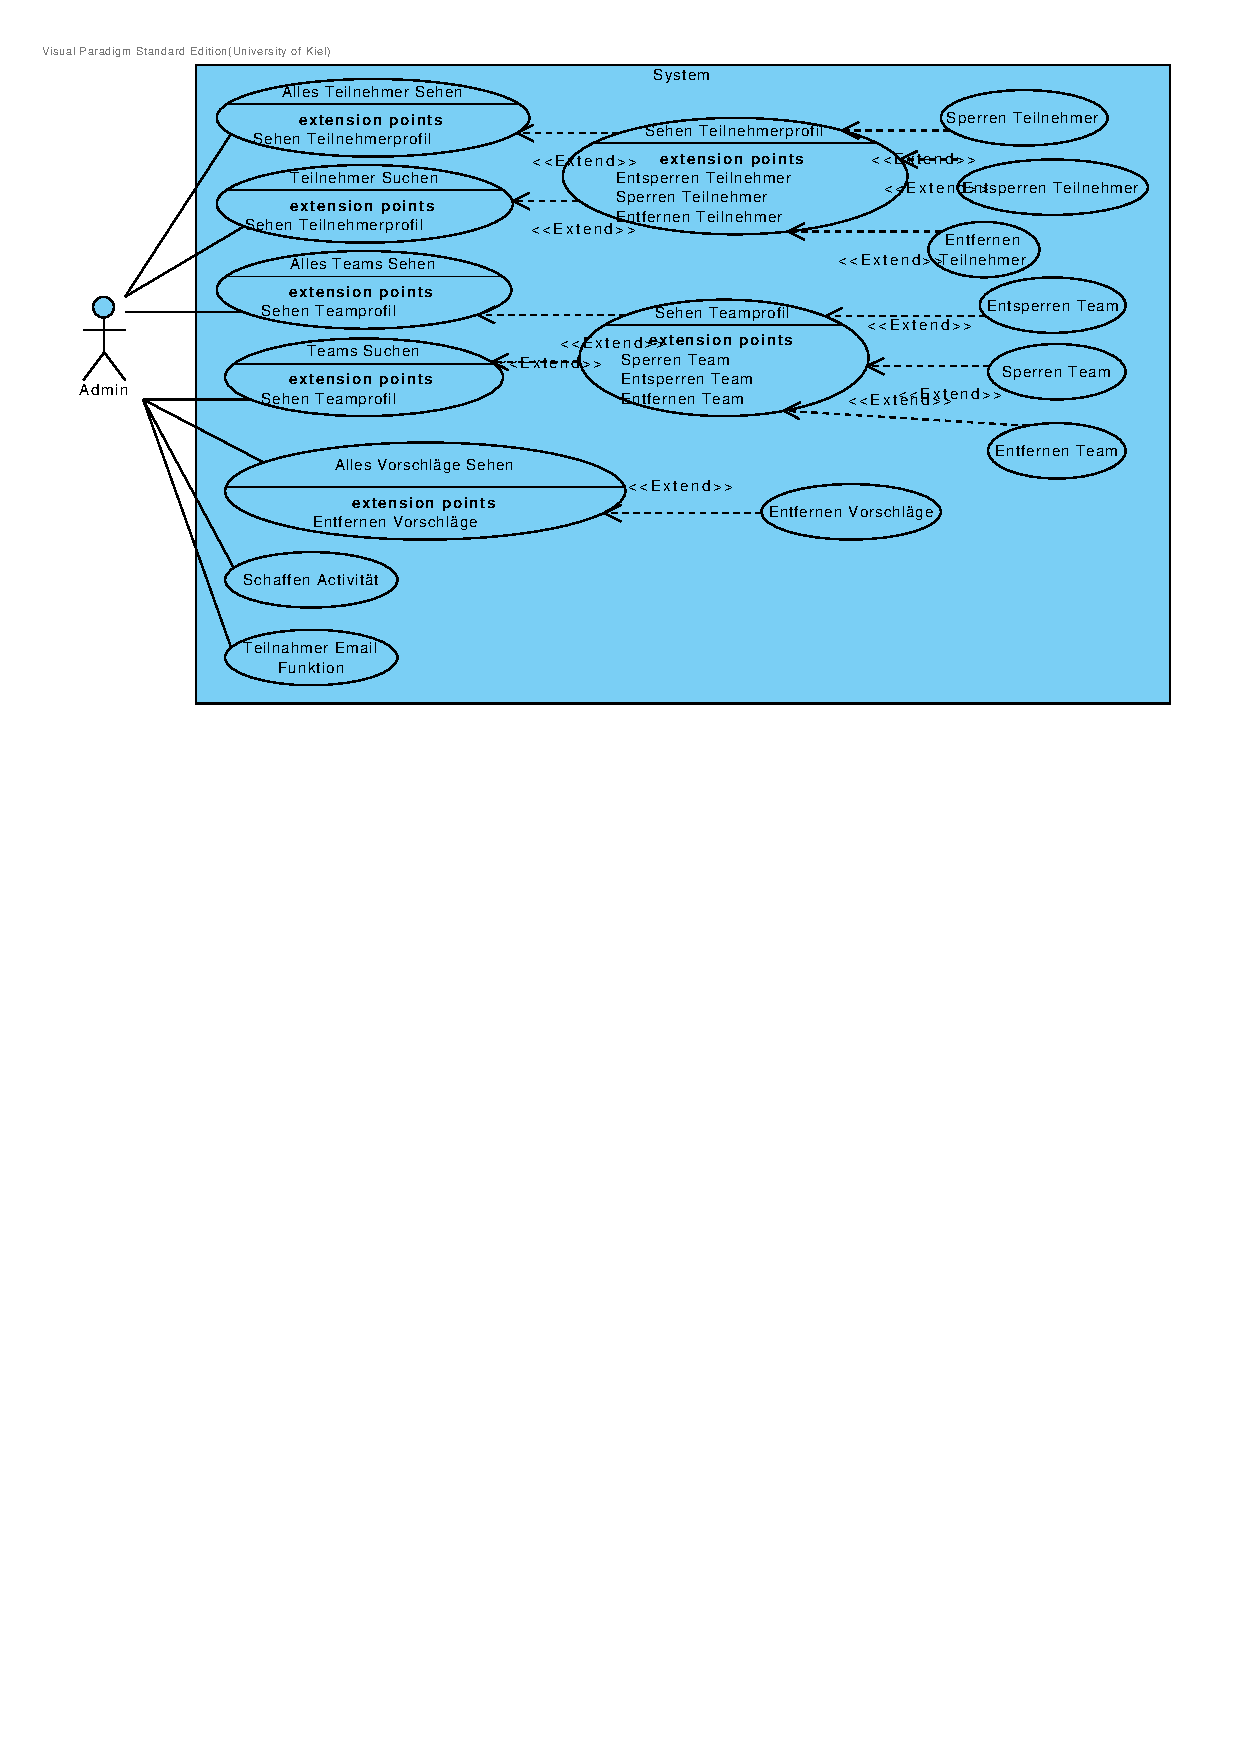
\includegraphics[width=\linewidth]{gfx/webseite/adminbereich.pdf}
	\end{figure}
	\begin{tabular}{|l|p{.5\linewidth}|}
	\hline Use Case Nummer & - \\ 
	\hline Use Case Name & Sperren Teilnehmer \\ 
	\hline Initiierender Akteur & Admin \\
	\hline Weitere Akteure & User \\
	\hline Kurzbeschreibung & The Administrator selects a user to be blocked who is then revoked access to the system. \\
	\hline Vorbedingung & Angelmeldet als Administrator \\
	\hline Nachbedingung &  \\
	\hline \multicolumn{2}{|c|}{Funktionalität des UseCases}\\
	\hline Ablauf & \begin{itemize}
			\item Admin locates the user on a list of all users.
			\item The Admin then selects the user to be blocked.
			\item The Admin must then confirm the blocking of that user.
		\end{itemize} \\ \\
	\hline Alternativen & \begin{itemize}
			\item Alternatively the users can be searched by the admin to find the correct selection.
		\end{itemize} \\
	\hline Ausnahmen &  \\
	\hline Benutzte Use Cases & \begin{itemize}
			\item Alles Teilnehmer Sehen
			\item Teilnehmer Suchen
			\item Sehen Teilnehmerprofil
		\end{itemize} \\
	\hline \multicolumn{2}{|c|}{Weitere Informationen} \\
	\hline Spezielle Anforderungen &  \\
	\hline Annahmen &  \\
	\hline
	\end{tabular}
	
	\subsubsection{Entsperren Teilnehmer}
	\begin{tabular}{|l|p{.5\linewidth}|}
	\hline Use Case Nummer & - \\ 
	\hline Use Case Name & Entsperren Teilnehmer \\ 
	\hline Initiierender Akteur & Admin \\
	\hline Weitere Akteure & User \\
	\hline Kurzbeschreibung & The Administrator selects a user who is currently blocked who is then allowed access to the system once again. \\
	\hline Vorbedingung & Angelmeldet als Administrator \\
	\hline Nachbedingung &  \\
	\hline \multicolumn{2}{|c|}{Funktionalität des UseCases}\\
	\hline Ablauf & \begin{itemize}
			\item Admin locates the user on a list of blocked users.
			\item The Admin then selects the user to be unblocked.
			\item The Admin must then confirm the unblocking of that user.
		\end{itemize} \\
	\hline Alternativen & \begin{itemize}
			\item Alternatively the users can be searched by the admin to find the correct selection.
		\end{itemize} \\
	\hline Ausnahmen &  \\
	\hline Benutzte Use Cases & \begin{itemize}
			\item Alles Teilnehmer Sehen
			\item Teilnehmer Suchen
			\item Sehen Teilnehmerprofil
		\end{itemize} \\
	\hline \multicolumn{2}{|c|}{Weitere Informationen} \\
	\hline Spezielle Anforderungen &  \\
	\hline Annahmen &  \\
	\hline
	\end{tabular}
	
	\subsubsection{Entfernen Teilnehmer}
	\begin{tabular}{|l|p{.5\linewidth}|}
	\hline Use Case Nummer & - \\ 
	\hline Use Case Name & Entfernen Teilnehmer \\ 
	\hline Initiierender Akteur & Admin \\
	\hline Weitere Akteure & User \\
	\hline Kurzbeschreibung & The Administrator selects a user and after confirming the selection that user account is deleted. \\
	\hline Vorbedingung & Angelmeldet als Administrator \\
	\hline Nachbedingung &  \\
	\hline \multicolumn{2}{|c|}{Funktionalität des UseCases}\\
	\hline Ablauf & \begin{itemize}
			\item Admin locates the user on a list of all users.
			\item The Admin then selects the user to be removed.
			\item The Admin must then confirm the complete removal of that user.
		\end{itemize} \\ \\
	\hline Alternativen & \begin{itemize}
			\item Alternatively the users can be searched by the admin to find the correct selection.
		\end{itemize} \\
	\hline Ausnahmen &  \\
	\hline Benutzte Use Cases & \begin{itemize}
			\item Alles Teilnehmer Sehen
			\item Teilnehmer Suchen
			\item Sehen Teilnehmerprofil
		\end{itemize} \\
	\hline \multicolumn{2}{|c|}{Weitere Informationen} \\
	\hline Spezielle Anforderungen &  \\
	\hline Annahmen &  \\
	\hline
	\end{tabular} 
	
	\subsubsection{Sperren Team}
	\begin{tabular}{|l|p{.5\linewidth}|}
	\hline Use Case Nummer & - \\ 
	\hline Use Case Name & Sperren Team \\ 
	\hline Initiierender Akteur & Admin \\
	\hline Weitere Akteure & User\\
	\hline Kurzbeschreibung & The Administrator selects a team to be blocked. That team is then no longer viewable on the system. \\
	\hline Vorbedingung & Angelmeldet als Administrator \\
	\hline Nachbedingung &  \\
	\hline \multicolumn{2}{|c|}{Funktionalität des UseCases}\\
	\hline Ablauf & \begin{itemize}
			\item Admin locates the team on a list of all teams.
			\item The Admin then selects the team to be blocked.
			\item The Admin must then confirm the blocking of that team.
		\end{itemize} \\ \\
	\hline Alternativen & \begin{itemize}
			\item Alternatively the teams can be searched by the admin to find the correct selection.
		\end{itemize} \\
	\hline Ausnahmen &  \\
	\hline Benutzte Use Cases & \begin{itemize}
			\item Alles Teams Sehen
			\item Teams Suchen
			\item Sehen Teamprofil
		\end{itemize} \\
	\hline \multicolumn{2}{|c|}{Weitere Informationen} \\
	\hline Spezielle Anforderungen &  \\
	\hline Annahmen &  \\
	\hline
	\end{tabular}
	
	\subsubsection{Entsperren Teilnehmer}
	\begin{tabular}{|l|p{.5\linewidth}|}
	\hline Use Case Nummer & - \\ 
	\hline Use Case Name & Entsperren Team \\ 
	\hline Initiierender Akteur & Admin \\
	\hline Weitere Akteure & User \\
	\hline Kurzbeschreibung & The Administrator selects a team who is currently blocked. That team is then viewable once again. \\
	\hline Vorbedingung & Angelmeldet als Administrator \\
	\hline Nachbedingung &  \\
	\hline \multicolumn{2}{|c|}{Funktionalität des UseCases}\\
	\hline Ablauf & \begin{itemize}
			\item Admin locates the team on a list of blocked teams.
			\item The Admin then selects the team to be unblocked.
			\item The Admin must then confirm the unblocking of that team.
		\end{itemize} \\ \\
	\hline Alternativen & \begin{itemize}
			\item Alternatively the teams can be searched by the admin to find the correct selection.
		\end{itemize} \\
	\hline Ausnahmen &  \\
	\hline Benutzte Use Cases & \begin{itemize}
			\item Alles Teams Sehen
			\item Teams Suchen
			\item Sehen Teamprofil
		\end{itemize} \\
	\hline \multicolumn{2}{|c|}{Weitere Informationen} \\
	\hline Spezielle Anforderungen &  \\
	\hline Annahmen &  \\
	\hline
	\end{tabular}
	
	\subsubsection{Entfernen Team}
	\begin{tabular}{|l|p{.5\linewidth}|}
	\hline Use Case Nummer & - \\ 
	\hline Use Case Name & Entfernen Team \\ 
	\hline Initiierender Akteur & Admin \\
	\hline Weitere Akteure & User \\
	\hline Kurzbeschreibung & The Administrator selects a team and after confirming the selection that team is deleted. \\
	\hline Vorbedingung & Angelmeldet als Administrator \\
	\hline Nachbedingung &  \\
	\hline \multicolumn{2}{|c|}{Funktionalität des UseCases}\\
	\hline Ablauf & \begin{itemize}
			\item Admin locates the team on a list of all team.
			\item The Admin then selects the user to be removed.
			\item The Admin must then confirm the complete removal of that team.
		\end{itemize} \\ \\
	\hline Alternativen & \begin{itemize}
			\item Alternatively the teams can be searched by the admin to find the correct selection.
		\end{itemize} \\
	\hline Ausnahmen &  \\
	\hline Benutzte Use Cases & \begin{itemize}
			\item Alles Teams Sehen
			\item Teams Suchen
			\item Sehen Teamprofil
		\end{itemize} \\
	\hline \multicolumn{2}{|c|}{Weitere Informationen} \\
	\hline Spezielle Anforderungen &  \\
	\hline Annahmen &  \\
	\hline
	\end{tabular}
	
	\subsubsection{Schaffen Activitat}
	\begin{tabular}{|l|p{.5\linewidth}|}
	\hline Use Case Nummer & - \\ 
	\hline Use Case Name & Schaffen Activitat \\ 
	\hline Initiierender Akteur & Admin \\
	\hline Weitere Akteure & \\
	\hline Kurzbeschreibung & The Admin fills out a form detailing a new activity which is then submitted to be used on the system. \\
	\hline Vorbedingung & Angelmeldet als Administrator \\
	\hline Nachbedingung &  \\
	\hline \multicolumn{2}{|c|}{Funktionalität des UseCases}\\
	\hline Ablauf & \begin{itemize}
			\item The Admin enters a title, description, points value, start date and end date.
			\item This information is then submitted and a new activity is created from the entered information.
		\end{itemize} \\ \\
	\hline Alternativen &  \\
	\hline Ausnahmen & \begin{itemize}
			\item The submission is rejected if any of the required information is not entered.
			\item The submission is rejected if the title or description are too long.
			\item The submission is rejected if the assinged points value is not a valid integer.
			\item The submission is rejected if the start and end dates are not in a valid date format.
		\end{itemize} \\
	\hline Benutzte Use Cases &  \\
	\hline \multicolumn{2}{|c|}{Weitere Informationen} \\
	\hline Spezielle Anforderungen &  \\
	\hline Annahmen & It is assumed that it is desirable for the admin to actully have validation imposed upon his entries. \\
	\hline
	\end{tabular}
	
	\subsubsection{Entfernen Vorschlage}
	\begin{tabular}{|l|p{.5\linewidth}|}
	\hline Use Case Nummer & - \\ 
	\hline Use Case Name & Entfernen Vorschlage \\ 
	\hline Initiierender Akteur & Admin \\
	\hline Weitere Akteure & \\
	\hline Kurzbeschreibung & The Administrator selects a team and after confirming the selection that team is deleted. \\
	\hline Vorbedingung & Angelmeldet als Administrator \\
	\hline Nachbedingung &  \\
	\hline \multicolumn{2}{|c|}{Funktionalität des UseCases}\\
	\hline Ablauf & \begin{itemize}
			\item Admin locates the proposal on a list of all proposals.
			\item The Admin then selects the proposal to be removed.
			\item The Admin must then confirm the complete removal of that proposal.
		\end{itemize} \\ \\
	\hline Alternativen &  \\
	\hline Ausnahmen &  \\
	\hline Benutzte Use Cases & \begin{itemize}
			\item Alles Vorschlage Sehen
		\end{itemize} \\
	\hline \multicolumn{2}{|c|}{Weitere Informationen} \\
	\hline Spezielle Anforderungen &  \\
	\hline Annahmen &  \\
	\hline
	\end{tabular}
	
\end{document}